\documentclass[aspectratio=169]{beamer}
\setbeamertemplate{navigation symbols}{} % don't use navigation tools on slides
% \usetheme{LMT}

\usepackage[utf8]{inputenc}
\usepackage{pdfpc-commands}
\usepackage{multimedia}
\usepackage{listings}
\usepackage{pgfplots}
\usepackage{default}
\usepackage{xcolor}

\setbeamersize{text margin left=0.6cm,text margin right=0.6cm}
\setbeamercolor{frametitle}{fg=black}
\setbeamercolor{section in toc}{fg=black}
\setbeamertemplate{frametitle}{\color{black}\bfseries\insertframetitle\par\vskip-6pt{\color{gray}\hrulefill}}

\lstset{language=C++,
  basicstyle=\ttfamily,
  keywordstyle=\color{blue}\ttfamily,
  stringstyle=\color{red}\ttfamily,
  commentstyle=\color{green}\ttfamily,
  morecomment=[l][\color{magenta}]{\#}
}

\AtBeginSection[]{
  \begin{frame}{Summary}
    \tableofcontents[currentsection]
  \end{frame} 
}

\begin{document}

\begin{frame}
    \begin{center}
        {\huge High Performance Computing of Power Diagrams}

        \bigskip
        {\large Applications to Semi-Discrete Optimal Transport}
      
        \vfill
        {(MAGA days, November 21, 2019, Hugo Leclerc)}
    \end{center}
\end{frame}

% ---------------------------------------------------------------------------------------
\section*{Introduction}

\begin{frame}
    \frametitle{The world needs power diagrams !}

    \begin{minipage}[c][0.6\textheight][c]{0.5\textwidth}
        Optimal way to transport a density to a set of diracs (equal mass) ? 
        
        \vfill
        Quadratic cost (euclidian distance) $\Rightarrow$ \textit{attributions} are defined by power diagrams !
        
        \vfill
        $x \in$ cell $i$ if $\forall j \neq i$,
         $$|| x - \rho_i ||^2 - \omega_i < || x - \rho_j ||^2 - \omega_j $$
    \end{minipage}
    \kern 0.5cm
    \begin{minipage}{0.45\textwidth}
        \begin{center}
            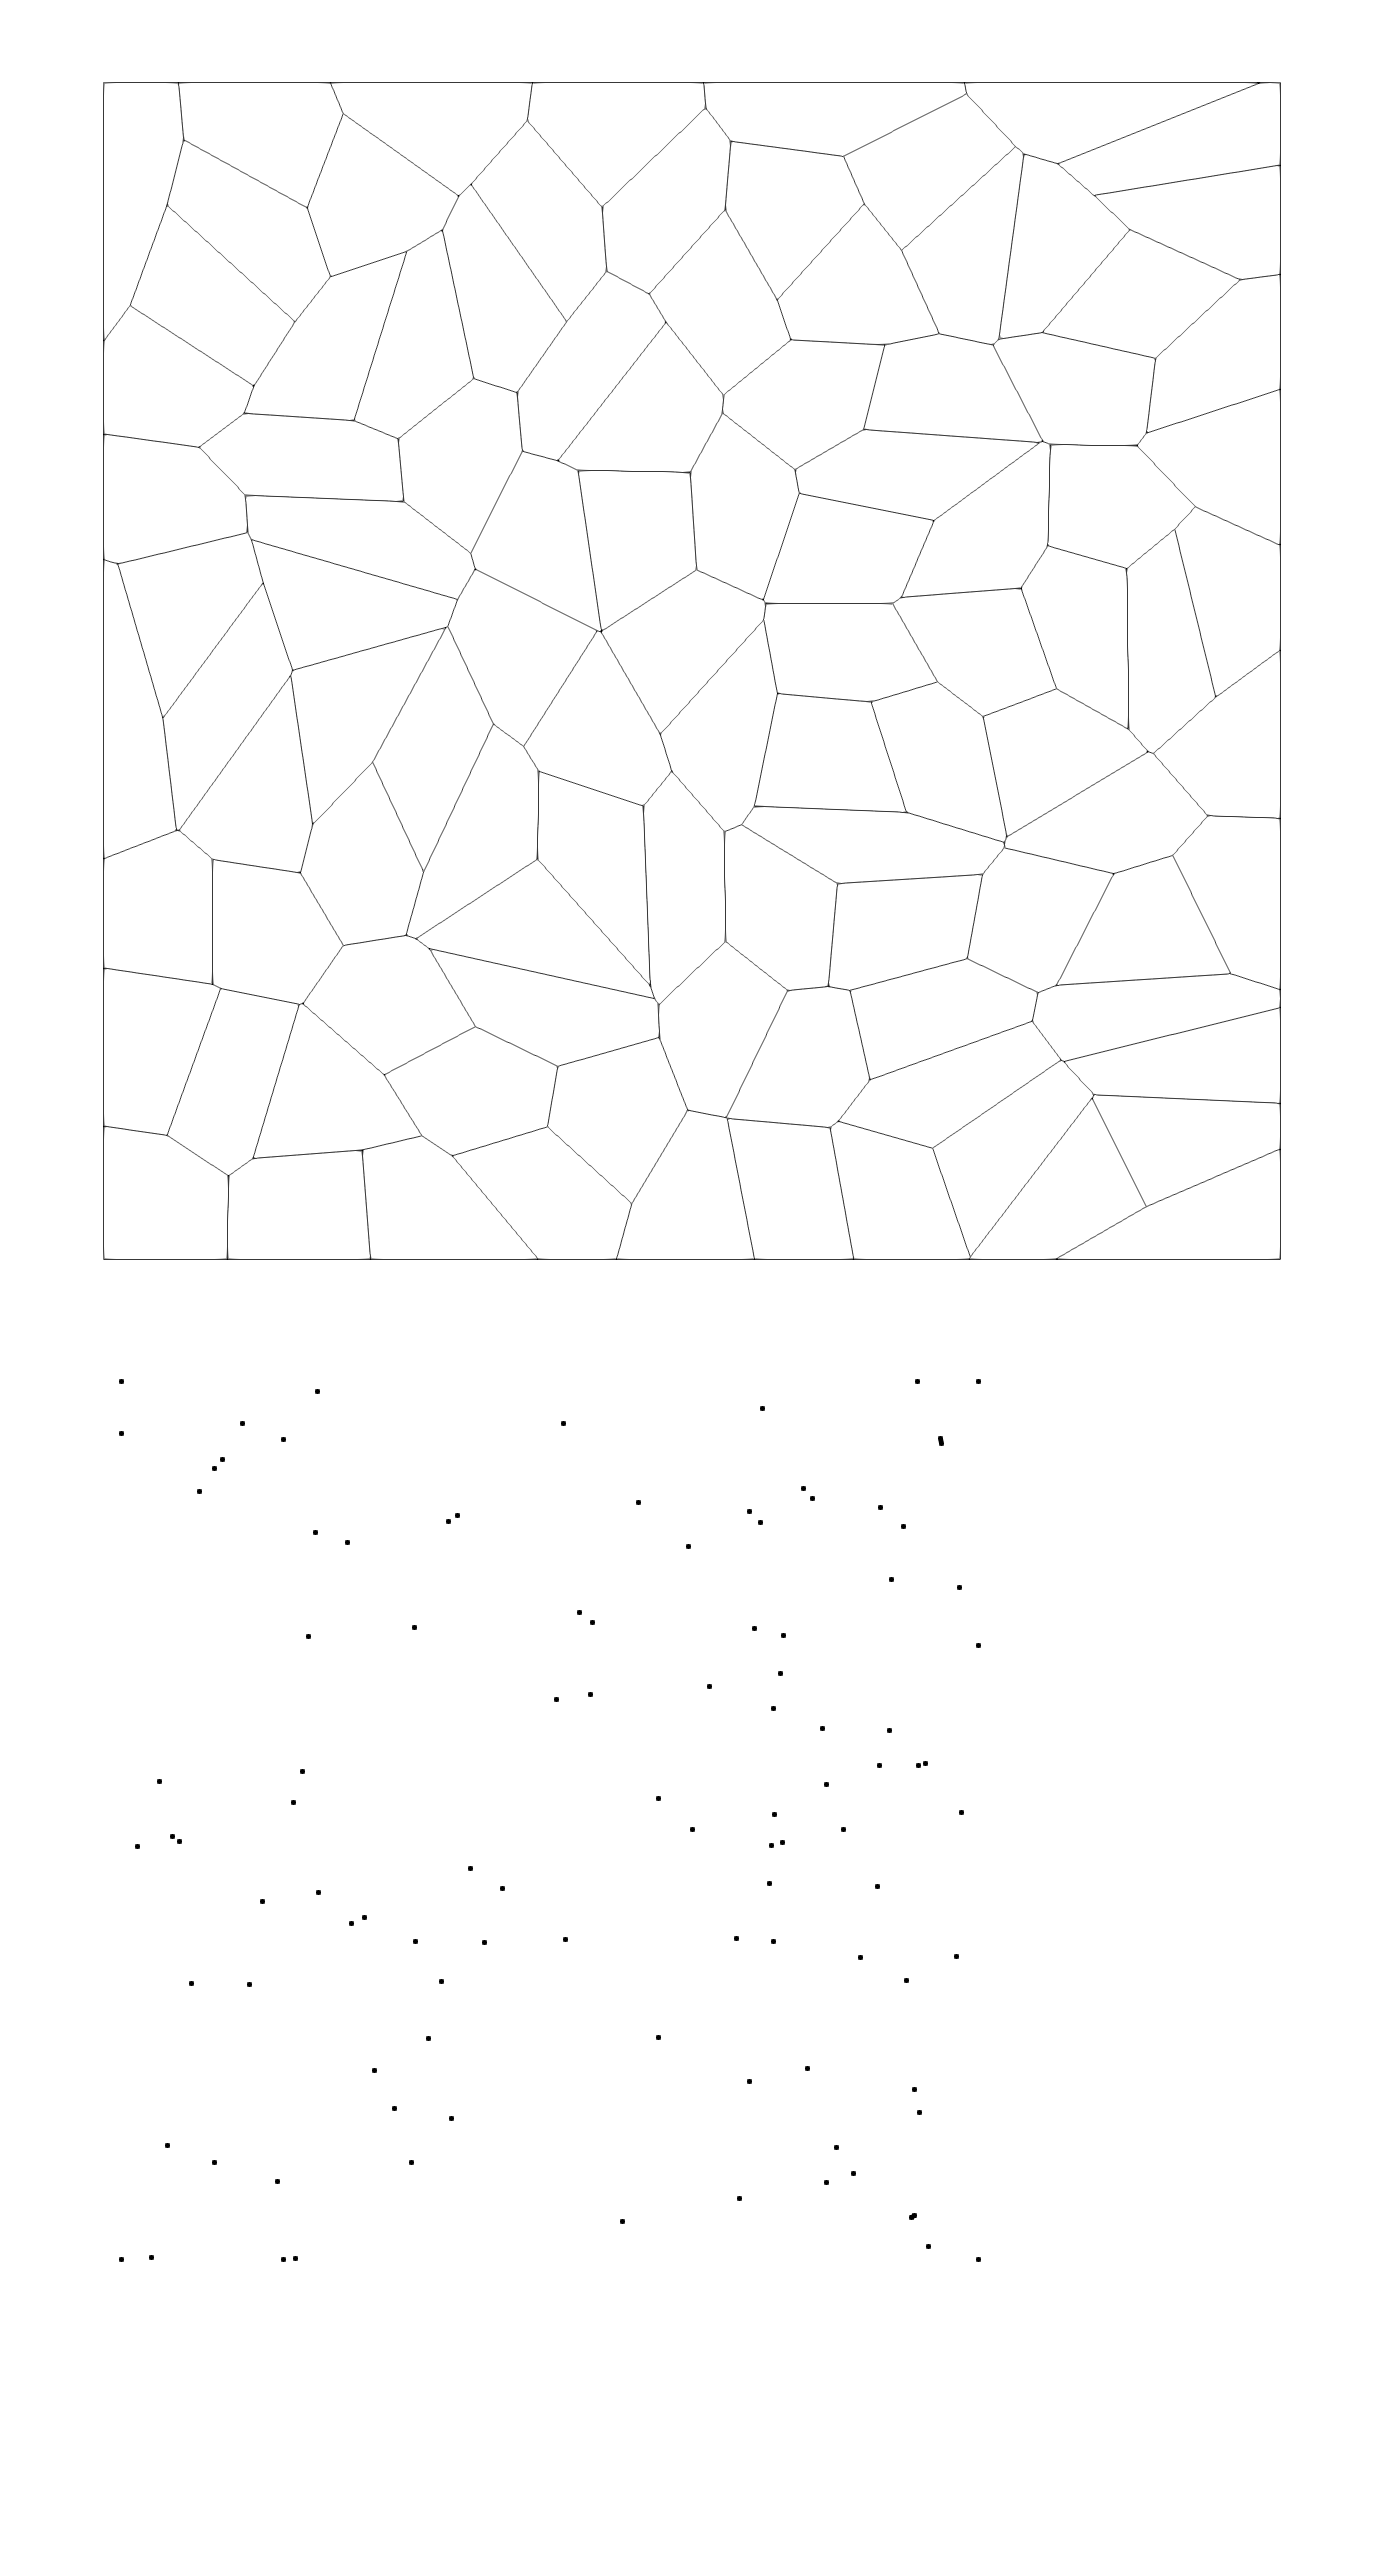
\includegraphics[height=0.8\textheight]{img/pd.png}
        \end{center}
    \end{minipage}
\end{frame}

\begin{frame}
    \frametitle{The world needs efficient power diagram computations !}

    Lot of work done before (Geogram, CGAL, ...), with a focus on the generic case.
    
    \vfill
    Most of the libraries are designed to give an \textit{exact connectivity}
    \begin{itemize}
        \item extra CPU and memory cost (bookkeeping)
        \item essentially sequential
    \end{itemize}

    \vfill
    SDOT application being more relaxed (need for simple integrals)
    \begin{itemize}
        \item development and test opportunities 
        \item scalability
    \end{itemize}
\end{frame}

\begin{frame}
    \frametitle{Individual cell computation}

    For each dirac $i$:
    \begin{itemize}
        \item starting from a non void finite cell (typically the domain boundaries),
        \item try some cuts with some \textit{close} diracs $j$
            \hfill{\textcolor{gray}{$\rightarrow$ Cell cuts}}

        \item until not possible to modify the cell
            \hfill{\textcolor{gray}{$\rightarrow$ Acceleration structures}}
    \end{itemize}
    
    \vfill
    Choices:
    \begin{itemize}
        \item infinite cells are handled by exceptions,
        \item tolerance on connectivity discrepancies (if zero mass),
        \item the sets of $j$ to test for a given $i$ are dynamic (dep. on updated cell geometry)
    \end{itemize}
    
\end{frame}

% ---------------------------------------------------------------------------------------
\section{Cell cuts}

\begin{frame}
    \frametitle{A word on test cases}

    Distributions
    \begin{itemize}
        \item uniform in $[0,1]^{dim}$,
        \item uniform in the faces of a Voronoï diagram with a fixed number of points (20),
    \end{itemize}

    \begin{center}
        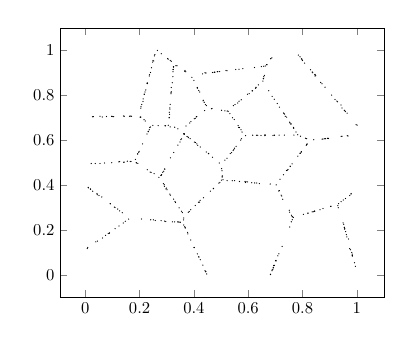
\begin{tikzpicture}[thick, scale=0.6]
  \begin{axis}
    \addplot [only marks, mark size=0.1pt] coordinates {
            ( 0.401544, 0.123371 )
            ( 0.377853, 0.18345 )
            ( 0.412696, 0.094736 )
            ( 0.367908, 0.211235 )
            ( 0.423769, 0.0686648 )
            ( 0.418974, 0.081198 )
            ( 0.376817, 0.190143 )
            ( 0.366483, 0.215511 )
            ( 0.444386, 0.0172317 )
            ( 0.362815, 0.222822 )
            ( 0.400546, 0.122734 )
            ( 0.440866, 0.0201061 )
            ( 0.433128, 0.0450913 )
            ( 0.388726, 0.156438 )
            ( 0.367847, 0.20972 )
            ( 0.417432, 0.0816121 )
            ( 0.44251, 0.0156105 )
            ( 0.447119, 0.00576412 )
            ( 0.0747329, 0.177071 )
            ( 0.00919154, 0.122965 )
            ( 0.0387603, 0.148201 )
            ( 0.159866, 0.249311 )
            ( 0.14745, 0.239462 )
            ( 0.139742, 0.231898 )
            ( 0.0449542, 0.15146 )
            ( 0.088092, 0.186434 )
            ( 0.0637233, 0.165528 )
            ( 0.12444, 0.218634 )
            ( 0.084978, 0.185211 )
            ( 0.10967, 0.206901 )
            ( 0.089022, 0.188134 )
            ( 0.00741753, 0.119004 )
            ( 0.0920801, 0.317235 )
            ( 0.0109817, 0.390008 )
            ( 0.011299, 0.387981 )
            ( 0.0439673, 0.357671 )
            ( 0.119323, 0.293905 )
            ( 0.0429018, 0.362898 )
            ( 0.061001, 0.347573 )
            ( 0.107255, 0.302591 )
            ( 0.0507313, 0.35375 )
            ( 0.13632, 0.277057 )
            ( 0.0918397, 0.317177 )
            ( 0.0190755, 0.381758 )
            ( 0.02746, 0.373235 )
            ( 0.109449, 0.300572 )
            ( 0.126635, 0.285666 )
            ( 0.0188767, 0.382924 )
            ( 0.362099, 0.245564 )
            ( 0.36272, 0.254164 )
            ( 0.349651, 0.235634 )
            ( 0.279251, 0.242196 )
            ( 0.292342, 0.240389 )
            ( 0.32916, 0.236807 )
            ( 0.250719, 0.24608 )
            ( 0.343366, 0.236085 )
            ( 0.240853, 0.246214 )
            ( 0.320898, 0.237004 )
            ( 0.29659, 0.238665 )
            ( 0.340185, 0.236596 )
            ( 0.25786, 0.243102 )
            ( 0.207233, 0.249925 )
            ( 0.348557, 0.235713 )
            ( 0.35744, 0.278164 )
            ( 0.287881, 0.406506 )
            ( 0.354158, 0.284218 )
            ( 0.332568, 0.322702 )
            ( 0.311538, 0.360218 )
            ( 0.330229, 0.327489 )
            ( 0.297141, 0.383311 )
            ( 0.345602, 0.299356 )
            ( 0.300887, 0.379342 )
            ( 0.313432, 0.355577 )
            ( 0.291518, 0.394532 )
            ( 0.290844, 0.401247 )
            ( 0.299599, 0.387113 )
            ( 0.325764, 0.337863 )
            ( 0.42289, 0.332439 )
            ( 0.388402, 0.290663 )
            ( 0.492044, 0.409178 )
            ( 0.379301, 0.279277 )
            ( 0.382741, 0.282647 )
            ( 0.435763, 0.344096 )
            ( 0.472659, 0.38579 )
            ( 0.501518, 0.422154 )
            ( 0.495689, 0.412113 )
            ( 0.46072, 0.37334 )
            ( 0.421067, 0.324555 )
            ( 0.471457, 0.383995 )
            ( 0.417274, 0.324305 )
            ( 0.405371, 0.309603 )
            ( 0.503962, 0.440295 )
            ( 0.503385, 0.46368 )
            ( 0.505547, 0.440522 )
            ( 0.504261, 0.435741 )
            ( 0.502188, 0.473228 )
            ( 0.235847, 0.645725 )
            ( 0.193568, 0.538155 )
            ( 0.231776, 0.639126 )
            ( 0.196664, 0.546065 )
            ( 0.237682, 0.65555 )
            ( 0.184627, 0.5142 )
            ( 0.240223, 0.658367 )
            ( 0.210942, 0.583013 )
            ( 0.231763, 0.637207 )
            ( 0.227269, 0.627243 )
            ( 0.192618, 0.53873 )
            ( 0.198327, 0.549974 )
            ( 0.242425, 0.456447 )
            ( 0.271217, 0.434741 )
            ( 0.239194, 0.457762 )
            ( 0.253525, 0.451026 )
            ( 0.188026, 0.498734 )
            ( 0.193552, 0.496707 )
            ( 0.228527, 0.468356 )
            ( 0.187737, 0.4998 )
            ( 0.281496, 0.446573 )
            ( 0.291954, 0.471644 )
            ( 0.313679, 0.521167 )
            ( 0.349106, 0.591581 )
            ( 0.325982, 0.544939 )
            ( 0.341471, 0.577581 )
            ( 0.278572, 0.443352 )
            ( 0.288869, 0.461714 )
            ( 0.363489, 0.627181 )
            ( 0.293188, 0.471166 )
            ( 0.354823, 0.605488 )
            ( 0.285621, 0.45732 )
            ( 0.364547, 0.626115 )
            ( 0.279549, 0.443197 )
            ( 0.352117, 0.601533 )
            ( 0.36294, 0.62782 )
            ( 0.364868, 0.627743 )
            ( 0.248791, 0.665193 )
            ( 0.268455, 0.663879 )
            ( 0.293726, 0.663089 )
            ( 0.295422, 0.66366 )
            ( 0.62384, 0.409627 )
            ( 0.522344, 0.419944 )
            ( 0.541253, 0.419339 )
            ( 0.631597, 0.409293 )
            ( 0.59233, 0.414986 )
            ( 0.589811, 0.411817 )
            ( 0.613001, 0.41051 )
            ( 0.567932, 0.416589 )
            ( 0.681065, 0.404703 )
            ( 0.597772, 0.414207 )
            ( 0.549887, 0.419916 )
            ( 0.641179, 0.407025 )
            ( 0.507048, 0.424134 )
            ( 0.588056, 0.416268 )
            ( 0.691789, 0.0328619 )
            ( 0.700765, 0.0650213 )
            ( 0.71307, 0.0952699 )
            ( 0.762318, 0.246425 )
            ( 0.702476, 0.0633627 )
            ( 0.693794, 0.0426857 )
            ( 0.687825, 0.0197334 )
            ( 0.693178, 0.0331661 )
            ( 0.694357, 0.0433754 )
            ( 0.682195, 0.00457597 )
            ( 0.702065, 0.0654758 )
            ( 0.688265, 0.023803 )
            ( 0.682097, 0.00291638 )
            ( 0.709139, 0.0862151 )
            ( 0.724989, 0.128042 )
            ( 0.752709, 0.214141 )
            ( 0.696754, 0.0438726 )
            ( 0.690764, 0.0260008 )
            ( 0.758737, 0.237057 )
            ( 0.954026, 0.21265 )
            ( 0.983216, 0.0937607 )
            ( 0.955186, 0.204367 )
            ( 0.983166, 0.0874571 )
            ( 0.952153, 0.226447 )
            ( 0.977038, 0.113283 )
            ( 0.973758, 0.11808 )
            ( 0.983633, 0.0885676 )
            ( 0.99487, 0.0394979 )
            ( 0.955631, 0.207233 )
            ( 0.983548, 0.0849575 )
            ( 0.954164, 0.2122 )
            ( 0.963397, 0.169964 )
            ( 0.930089, 0.308852 )
            ( 0.981456, 0.100674 )
            ( 0.961578, 0.180311 )
            ( 0.949485, 0.232201 )
            ( 0.991519, 0.0558627 )
            ( 0.96926, 0.160972 )
            ( 0.959128, 0.193755 )
            ( 0.932, 0.299507 )
            ( 0.8394, 0.282164 )
            ( 0.820604, 0.27626 )
            ( 0.904837, 0.305981 )
            ( 0.835659, 0.281202 )
            ( 0.766157, 0.256789 )
            ( 0.820127, 0.27451 )
            ( 0.864252, 0.290873 )
            ( 0.903651, 0.305434 )
            ( 0.803357, 0.27037 )
            ( 0.875614, 0.295951 )
            ( 0.844159, 0.285112 )
            ( 0.844939, 0.283784 )
            ( 0.95015, 0.334219 )
            ( 0.979216, 0.362321 )
            ( 0.942026, 0.326721 )
            ( 0.974251, 0.353962 )
            ( 0.932835, 0.317789 )
            ( 0.958299, 0.340723 )
            ( 0.978315, 0.360559 )
            ( 0.884245, 0.606443 )
            ( 0.891557, 0.607704 )
            ( 0.942423, 0.616458 )
            ( 0.967625, 0.617838 )
            ( 0.895772, 0.606694 )
            ( 0.893906, 0.607724 )
            ( 0.875263, 0.60455 )
            ( 0.945237, 0.616763 )
            ( 0.872203, 0.604342 )
            ( 0.965179, 0.619194 )
            ( 0.841707, 0.601548 )
            ( 0.882373, 0.605821 )
            ( 0.746442, 0.469522 )
            ( 0.795586, 0.548738 )
            ( 0.761518, 0.494455 )
            ( 0.817778, 0.582594 )
            ( 0.795023, 0.546448 )
            ( 0.716998, 0.426331 )
            ( 0.74076, 0.464931 )
            ( 0.815279, 0.581391 )
            ( 0.81376, 0.577051 )
            ( 0.78282, 0.528539 )
            ( 0.75481, 0.484307 )
            ( 0.754957, 0.482656 )
            ( 0.744571, 0.46664 )
            ( 0.79207, 0.541661 )
            ( 0.729761, 0.446162 )
            ( 0.790933, 0.541149 )
            ( 0.721396, 0.355263 )
            ( 0.714664, 0.375457 )
            ( 0.762837, 0.259288 )
            ( 0.70329, 0.401117 )
            ( 0.752627, 0.279839 )
            ( 0.723582, 0.351962 )
            ( 0.712755, 0.374192 )
            ( 0.727187, 0.337015 )
            ( 0.76184, 0.260274 )
            ( 0.759779, 0.266281 )
            ( 0.75133, 0.288826 )
            ( 0.126631, 0.50427 )
            ( 0.0219588, 0.495596 )
            ( 0.1238, 0.503108 )
            ( 0.0707419, 0.498496 )
            ( 0.141742, 0.501595 )
            ( 0.168433, 0.504859 )
            ( 0.165371, 0.504858 )
            ( 0.154912, 0.50624 )
            ( 0.0367013, 0.495782 )
            ( 0.143057, 0.502117 )
            ( 0.0976184, 0.499602 )
            ( 0.0539518, 0.49599 )
            ( 0.202376, 0.702544 )
            ( 0.202425, 0.701607 )
            ( 0.204523, 0.701866 )
            ( 0.220787, 0.684711 )
            ( 0.216545, 0.690528 )
            ( 0.166139, 0.706622 )
            ( 0.143557, 0.706054 )
            ( 0.0267046, 0.703742 )
            ( 0.0995202, 0.704468 )
            ( 0.104638, 0.703874 )
            ( 0.0299945, 0.703735 )
            ( 0.0975065, 0.705239 )
            ( 0.140717, 0.707121 )
            ( 0.162793, 0.705764 )
            ( 0.0626189, 0.702819 )
            ( 0.0544615, 0.705466 )
            ( 0.170183, 0.705884 )
            ( 0.0783252, 0.704276 )
            ( 0.227442, 0.852155 )
            ( 0.252418, 0.951249 )
            ( 0.24355, 0.921 )
            ( 0.207811, 0.758045 )
            ( 0.212675, 0.771565 )
            ( 0.228652, 0.853504 )
            ( 0.20471, 0.741552 )
            ( 0.205426, 0.747797 )
            ( 0.219948, 0.813662 )
            ( 0.217626, 0.802855 )
            ( 0.256353, 0.978895 )
            ( 0.254649, 0.973746 )
            ( 0.236782, 0.890044 )
            ( 0.24976, 0.953314 )
            ( 0.247804, 0.946085 )
            ( 0.229057, 0.850785 )
            ( 0.216839, 0.803914 )
            ( 0.222933, 0.822658 )
            ( 0.240582, 0.900001 )
            ( 0.235935, 0.884353 )
            ( 0.213182, 0.782587 )
            ( 0.386254, 0.606216 )
            ( 0.374975, 0.61593 )
            ( 0.380134, 0.610852 )
            ( 0.453465, 0.540458 )
            ( 0.414557, 0.577026 )
            ( 0.405887, 0.589332 )
            ( 0.410824, 0.583039 )
            ( 0.377717, 0.614408 )
            ( 0.423645, 0.569062 )
            ( 0.493682, 0.49805 )
            ( 0.445692, 0.547098 )
            ( 0.4018, 0.590995 )
            ( 0.454538, 0.539516 )
            ( 0.468774, 0.523924 )
            ( 0.544656, 0.553503 )
            ( 0.514234, 0.510915 )
            ( 0.575366, 0.606173 )
            ( 0.55531, 0.572009 )
            ( 0.547039, 0.557562 )
            ( 0.522118, 0.519393 )
            ( 0.549532, 0.56417 )
            ( 0.538893, 0.544293 )
            ( 0.572281, 0.599971 )
            ( 0.533745, 0.540201 )
            ( 0.573656, 0.645685 )
            ( 0.567938, 0.655333 )
            ( 0.542514, 0.698922 )
            ( 0.548485, 0.691241 )
            ( 0.526381, 0.727404 )
            ( 0.564607, 0.656253 )
            ( 0.532765, 0.717387 )
            ( 0.577354, 0.635459 )
            ( 0.56296, 0.664481 )
            ( 0.522715, 0.728719 )
            ( 0.465065, 0.738854 )
            ( 0.466651, 0.740319 )
            ( 0.501765, 0.731892 )
            ( 0.514244, 0.729992 )
            ( 0.308883, 0.698685 )
            ( 0.311658, 0.737725 )
            ( 0.325499, 0.924726 )
            ( 0.316839, 0.814053 )
            ( 0.305846, 0.665818 )
            ( 0.311451, 0.742814 )
            ( 0.322728, 0.881366 )
            ( 0.315622, 0.80586 )
            ( 0.309331, 0.700085 )
            ( 0.32328, 0.913849 )
            ( 0.323665, 0.913136 )
            ( 0.316736, 0.833013 )
            ( 0.320356, 0.854312 )
            ( 0.312889, 0.758499 )
            ( 0.310448, 0.714269 )
            ( 0.322935, 0.903516 )
            ( 0.32489, 0.924861 )
            ( 0.324802, 0.92475 )
            ( 0.315894, 0.81202 )
            ( 0.309572, 0.723667 )
            ( 0.341069, 0.650054 )
            ( 0.329154, 0.656995 )
            ( 0.312804, 0.658476 )
            ( 0.408963, 0.70419 )
            ( 0.409781, 0.704002 )
            ( 0.405166, 0.696902 )
            ( 0.410735, 0.703267 )
            ( 0.389204, 0.681986 )
            ( 0.385036, 0.675703 )
            ( 0.439578, 0.730936 )
            ( 0.401102, 0.694655 )
            ( 0.371161, 0.662609 )
            ( 0.412273, 0.831399 )
            ( 0.418011, 0.820279 )
            ( 0.412388, 0.833111 )
            ( 0.413483, 0.830923 )
            ( 0.434434, 0.776948 )
            ( 0.400167, 0.864723 )
            ( 0.446135, 0.753266 )
            ( 0.442439, 0.757483 )
            ( 0.392825, 0.878429 )
            ( 0.438169, 0.767359 )
            ( 0.42182, 0.81352 )
            ( 0.434139, 0.774113 )
            ( 0.337646, 0.929977 )
            ( 0.370215, 0.903588 )
            ( 0.367399, 0.908938 )
            ( 0.334111, 0.93035 )
            ( 0.366513, 0.905442 )
            ( 0.316725, 0.950053 )
            ( 0.305225, 0.959296 )
            ( 0.265804, 0.997924 )
            ( 0.279811, 0.982784 )
            ( 0.312973, 0.952887 )
            ( 0.303629, 0.961575 )
            ( 0.545468, 0.752474 )
            ( 0.615871, 0.81843 )
            ( 0.626773, 0.830187 )
            ( 0.628511, 0.834345 )
            ( 0.574442, 0.778481 )
            ( 0.637292, 0.845044 )
            ( 0.566513, 0.772484 )
            ( 0.551851, 0.757924 )
            ( 0.561549, 0.764178 )
            ( 0.628657, 0.832027 )
            ( 0.603578, 0.806105 )
            ( 0.614241, 0.818424 )
            ( 0.597666, 0.8033 )
            ( 0.630783, 0.621532 )
            ( 0.662671, 0.620973 )
            ( 0.691359, 0.6204 )
            ( 0.616435, 0.621463 )
            ( 0.695789, 0.621796 )
            ( 0.59023, 0.619744 )
            ( 0.661781, 0.623277 )
            ( 0.661416, 0.619688 )
            ( 0.647125, 0.620088 )
            ( 0.73325, 0.622112 )
            ( 0.635492, 0.621559 )
            ( 0.713772, 0.621907 )
            ( 0.69711, 0.621246 )
            ( 0.768475, 0.622224 )
            ( 0.475844, 0.901153 )
            ( 0.441347, 0.898753 )
            ( 0.474668, 0.900709 )
            ( 0.580411, 0.91679 )
            ( 0.486228, 0.903614 )
            ( 0.663074, 0.928631 )
            ( 0.518028, 0.908771 )
            ( 0.432092, 0.893721 )
            ( 0.495052, 0.904009 )
            ( 0.48811, 0.903767 )
            ( 0.522303, 0.907705 )
            ( 0.554461, 0.913063 )
            ( 0.566033, 0.914361 )
            ( 0.468595, 0.899643 )
            ( 0.444289, 0.897653 )
            ( 0.477469, 0.901822 )
            ( 0.623031, 0.922159 )
            ( 0.657232, 0.927515 )
            ( 0.648618, 0.926383 )
            ( 0.815331, 0.606214 )
            ( 0.792884, 0.61728 )
            ( 0.811107, 0.608383 )
            ( 0.837871, 0.8985 )
            ( 0.867214, 0.856023 )
            ( 1.00109, 0.666276 )
            ( 0.997418, 0.668451 )
            ( 0.928938, 0.770271 )
            ( 0.942013, 0.755757 )
            ( 0.846155, 0.884908 )
            ( 0.800111, 0.953515 )
            ( 0.95811, 0.726328 )
            ( 0.919799, 0.780482 )
            ( 0.845512, 0.890326 )
            ( 0.797122, 0.959784 )
            ( 0.848916, 0.885641 )
            ( 0.926817, 0.773009 )
            ( 0.796013, 0.960777 )
            ( 0.955369, 0.73028 )
            ( 0.964298, 0.719443 )
            ( 0.883279, 0.834579 )
            ( 0.807908, 0.941779 )
            ( 0.846394, 0.891378 )
            ( 0.790886, 0.969376 )
            ( 0.953755, 0.732249 )
            ( 0.907572, 0.799682 )
            ( 0.835753, 0.901824 )
            ( 0.798526, 0.956175 )
            ( 0.872049, 0.849825 )
            ( 0.82955, 0.912344 )
            ( 0.784679, 0.977251 )
            ( 0.945447, 0.742717 )
            ( 0.669659, 0.934312 )
            ( 0.683195, 0.960629 )
            ( 0.667696, 0.934703 )
            ( 0.687384, 0.964955 )
            ( 0.683461, 0.961691 )
            ( 0.654253, 0.861951 )
            ( 0.656709, 0.872887 )
            ( 0.655522, 0.872552 )
            ( 0.659996, 0.887117 )
            ( 0.657666, 0.880946 )
            ( 0.782583, 0.623616 )
            ( 0.776121, 0.63569 )
            ( 0.696013, 0.781282 )
            ( 0.767663, 0.6523 )
            ( 0.730099, 0.72007 )
            ( 0.736858, 0.705758 )
            ( 0.752703, 0.679175 )
            ( 0.754055, 0.675783 )
            ( 0.757818, 0.67207 )
            ( 0.688233, 0.793702 )
            ( 0.731753, 0.717696 )
            ( 0.714923, 0.745965 )
            ( 0.67594, 0.818907 )
            ( 0.757304, 0.670805 )
            ( 0.767296, 0.656222 )
            ( 0.766483, 0.653808 )
            ( 0.741683, 0.70206 )
            ( 0.707121, 0.762002 )
            ( 0.733877, 0.715258 )
    };
  \end{axis}
\end{tikzpicture}

        \kern 1cm
        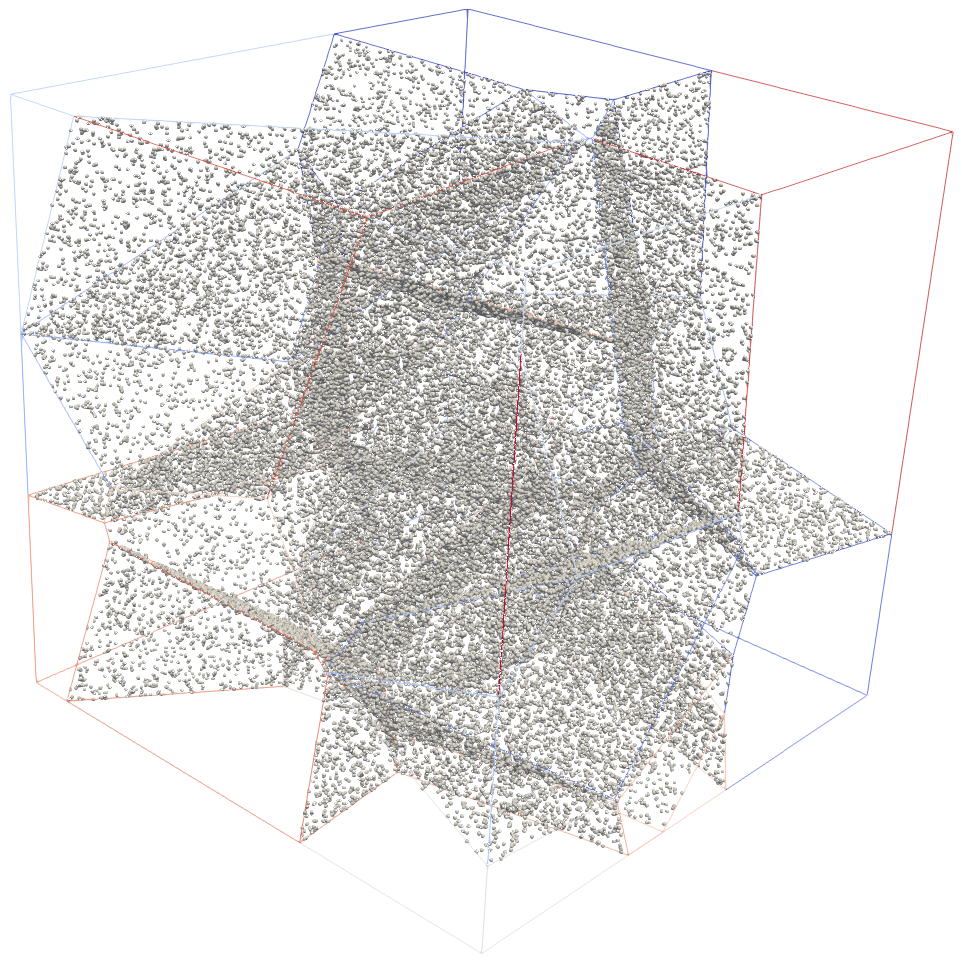
\includegraphics[width=0.26\textwidth]{img/voro_distrib_3d.png}
    \end{center}


    \vfill
    Focus on the time to construct the cells.
\end{frame}

\begin{frame}
    \frametitle{Distribution $\#$ nodes / cell before each cut, 2D case}

    \begin{minipage}[c][0.6\textheight][c]{0.4\textwidth}
            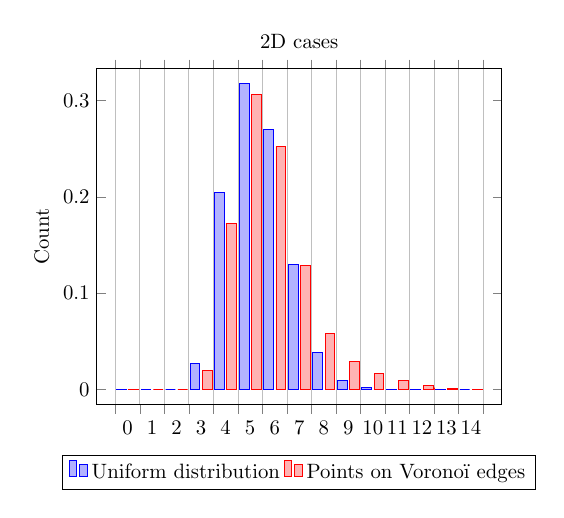
\begin{tikzpicture}[scale=0.75]
    \begin{axis}[
        legend style={at={(0.5,-0.15)},anchor=north,legend columns=-1},
        ybar interval=0.8,
        ylabel=Count,
        title=2D cases,
        enlargelimits=0.05,
    ]
    \addplot coordinates {
       ( 0, 1.58049e-06 )           
       ( 1, 0           )
       ( 2, 0           )
       ( 3, 0.0269854   )         
       ( 4, 0.204727    )        
       ( 5, 0.317403    )        
       ( 6, 0.270196    )        
       ( 7, 0.129706    )        
       ( 8, 0.0389355   )         
       ( 9, 0.00941079  )          
       (10, 0.00214473  )          
       (11, 0.000444119 )           
       (12, 4.47807e-05 )
       (13, 2.10733e-06 )
       (14, 0           )
       (15, 0           )
       % (16, 0           )
       % (17, 0           )
       % (18, 0           )
       % (19, 0           )
    };
    \addplot coordinates {
       ( 0, 7.68332e-06 )
       ( 1, 0           )
       ( 2, 0           )
       ( 3, 0.0202567   )
       ( 4, 0.172274    )
       ( 5, 0.306317    )
       ( 6, 0.252301    )
       ( 7, 0.128378    )
       ( 8, 0.0579965   )
       ( 9, 0.028838    )
       (10, 0.0167608   )
       (11, 0.00910499  )
       (12, 0.00417465  )
       (13, 0.00208543  )
       (13, 0.000886446 )
       (14, 0.00030603  )
       (15, 0.000186223 )
       % (16, 8.26933e-05 )
       % (17, 3.29471e-05 )
       % (18, 7.55309e-06 )
       % (19, 3.51609e-06 )
    };
    \legend{Uniform distribution,Points on Voronoï edges}
    \end{axis}
\end{tikzpicture}

    \end{minipage}
    \kern 0.04\textwidth
    \begin{minipage}{0.55\textwidth}
        \begin{itemize}
            \item Obvious
        \end{itemize}
    \end{minipage}
\end{frame}



\begin{frame}
    \frametitle{Distribution $\#$ nodes / cell before each cut, 3D case}
    \begin{center}
        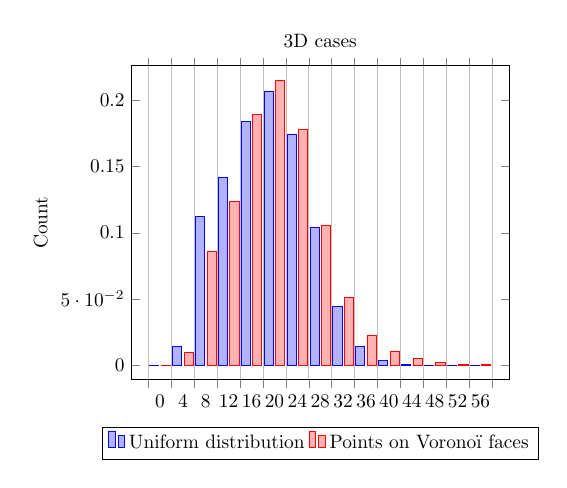
\begin{tikzpicture}[scale=0.7]
    \begin{axis}[
        legend style={at={(0.5,-0.15)},anchor=north,legend columns=-1},
        ybar interval=0.8,
        ylabel=Count,
        title=3D cases,
        enlargelimits=0.05,
    ]
    \addplot coordinates {
        (  0, 8.486250e-07 )
        (  4, 1.407526e-02 )
        (  8, 1.121475e-01 )
        ( 12, 1.418800e-01 )
        ( 16, 1.838793e-01 )
        ( 20, 2.061940e-01 )
        ( 24, 1.739535e-01 )
        ( 28, 1.041492e-01 )
        ( 32, 4.463720e-02 )
        ( 36, 1.415705e-02 )
        ( 40, 3.759130e-03 )
        ( 44, 8.953000e-04 )
        ( 48, 2.305428e-04 )
        ( 52, 2.970185e-05 )
        ( 56, 5.657500e-06 )
        ( 60, 1.697250e-06 )
        %(  0, 8.48625e-07 )
        %(  2, 0           )
        %(  4, 0.00166076  )
        %(  6, 0.0124145   )
        %(  8, 0.055026    )
        %( 10, 0.0571215   )
        %( 12, 0.0658276   )
        %( 14, 0.0760524   )
        %( 16, 0.0868673   )
        %( 18, 0.097012    )
        %( 20, 0.102684    )
        %( 22, 0.10351     )
        %( 24, 0.0937935   )
        %( 26, 0.08016     )
        %( 28, 0.0611126   )
        %( 30, 0.0430366   )
        %( 32, 0.027646    )
        %( 34, 0.0169912   )
        %( 36, 0.00930461  )
        %( 38, 0.00485244  )
        %( 40, 0.00249666  )
        %( 42, 0.00126247  )
        %( 44, 0.000582723 )
        %( 46, 0.000312577 )
        %( 48, 0.00016435  )
        %( 50, 6.61928e-05 )
        %( 52, 2.00841e-05 )
        %( 54, 9.61775e-06 )
        %( 56, 2.82875e-06 )
        %( 58, 2.82875e-06 )
        %( 60, 8.48625e-07 )
        %( 62, 8.48625e-07 )
        %( 64, 4.526e-06   )
    };
    \addplot coordinates {
        (  0, 1.505050e-06 )
        (  4, 9.766150e-03 )
        (  8, 8.581940e-02 )
        ( 12, 1.237691e-01 )
        ( 16, 1.892904e-01 )
        ( 20, 2.150680e-01 )
        ( 24, 1.776119e-01 )
        ( 28, 1.058479e-01 )
        ( 32, 5.102420e-02 )
        ( 36, 2.251171e-02 )
        ( 40, 1.034158e-02 )
        ( 44, 4.915620e-03 )
        ( 48, 2.280648e-03 )
        ( 52, 1.025441e-03 )
        ( 56, 4.561560e-04 )
        ( 60, 1.724536e-04 )
        % ( 64, 5.869700e-05 )
        % ( 68, 2.433162e-05 )
        % ( 72, 1.028451e-05 )
        % ( 76, 3.135520e-06 )
    };
    \legend{Uniform distribution,Points on Voronoï faces}
    \end{axis}
\end{tikzpicture}

    \end{center}

    \vfill
    Pouet
\end{frame}


% ---------------------------------------------------------------------------------------
\section{Acceleration structures}

\begin{frame}
    \frametitle{Focus on parallel cell computations}

    Basically a $\mathcal{O}( n^2 )$ algorithm ($\forall\ i, j \neq i$)
    
    
\end{frame}


% ---------------------------------------------------------------------------------------
\section{Product placement}


% ---------------------------------------------------------------------------------------
\section{Conclusions}

\begin{frame}
    \frametitle{Conclusions}

    Smurf
    \begin{itemize}
        \item ...
    \end{itemize}
    
    \vfill
\end{frame}


\begin{frame}
    \frametitle{Perspectives}

\end{frame}


\end{document}
